\input{../header.tex}

\subject{VERSUCH NUMMER 601}
\title{Franck-Hertz-Versuch}
\date{
  Durchführung: 09.05.2023
  \hspace{3em}
  Abgabe: 16.05.2023
}

\begin{document}

\maketitle
\thispagestyle{empty}
\tableofcontents
\newpage
\setcounter{page}{1}
\section{Ziel}
\label{sec:Ziel}

Mittels des Franck-Hertz-Versuchs gelang es 1914 eine Anregungsenergie des Quecksilber-Atoms zu bestimmen sowie einen Zusammenhang zwischen 
dieser und der Wellenlänge des emittierten Lichts herzustellen. Außerdem konnten die Bohrschen Postulate zum Aufbau der Elektronenhülle teilweise bestätigt 
werden. 

In diesem Versuch soll die Energieverteilung der verwendeten Elektronen und die Ionisierungsenergie von Quecksilber bestimmt werden. Zusätzlich 
dazu werden mehrere Franck-Hertz-Kurven bestimmt, um die Anregungsenergie des Hg-Atoms zu bestimmen
\section{Theorie}
\label{sec:Theorie}

Der Franck-Hertz-Versuch gehört zu den Elektronenstoßexperimenten. Dabei werden in einem mit Hg-Dampf gefüllten Glaskolben die Hg-Atome mit Elektronen 
sowohl elastisch wie unelastisch gestoßen. Die Elektronen werden dabei mittels eines Glühdrahtes erzeugt, welcher zusätzlich mit einem Oxid eines 
Erdalkalimetalles bestrichen wird, sodass die Austrittsarbeit niedrig ist und selbst bei geringer Temperatur viele Elektronen emittiert werden.
Um die Energiedifferenz zwischen dem ersten angeregten Zustand und dem Grundzustand zu messen, kann die 
Energiedifferenz der Elektronen vor und nach einem unelastischen Stoß beobachtet werden. Es gilt für die Energiedifferenz der Zustände
\begin{equation*}
    \frac{m_0\cdot v^2_{\symup{vor}}}{2} - \frac{m_0\cdot v^2_{\symup{nach}}}{2} = E_1 - E_0 \; .
\end{equation*}

Gegenüber des Glühdrahtes befindet sich eine netzförmige Elektrode, die die Elektronen mittels einer Gleichspannung $U_{\symup{B}}$ beschleunigt. 
Die kinetische Energie der Elektronen lässt sich über 
\begin{equation*}
    \frac{m_0\cdot v^2_{\symup{vor}}}{2} = e_0U_{\symup{B}}
\end{equation*}
beschreiben.
Hinter der Beschleunigungselektrode befindet sich die Auffängerelektrode, auf der die Elektronen landen und einen Auffängerstrom $I_{\symup{A}}$ erzeugen.
Die Auffängerelektrode besitzt jedoch eine geringe Gegenspannung $U_{\symup{A}}$, durch die Elektronen ein Bremsfeld überwinden müssen. Nur Elektronen, 
die die Ungleichung
\begin{equation*}
    \frac{m_0}{2}v^2_{\symup{z}} \geq e_0U_{\symup{A}}
\end{equation*}
erfüllen, erreichen somit die Auffängerelektrode. 

Im Beschleunigungsraum befinden sich nun Hg-Atome, die mit den Elektronen zusammenstoßen können. Dabei ist zwischen elastischen und unelastischen Stößen 
zu unterscheiden. Wenn die Elektronenenergie gering ist, sind alle Stöße elastisch. Die Energieabgabe des Elektrons and das Hg-Atom ist jedoch aufgrund 
der hohen Massendifferenz vernachlässigbar klein. Die Richtungsänderung des Elektrons kann jedoch erheblich sein. 
Wenn die Elektronendifferenz größer oder gleich der Energiedifferenz $E_1 - E_0$ ist, kann das Elektron das Hg-Atom anregen. Dabei wird die eben 
genannte Energiedifferenz auf das Hg-Atom übertragen und dieses befindet sich im ersten angeregten Zustand. Nach einer kurzen Relaxationszeit, fällt
das Hg-Atom in den Grundzustand zurück und emittiert dabei ein Photon mit eben dieser Energiedifferenz
\begin{equation}
    \symup{h}\nu = E_1 - E_0 \; .
    \label{eqn:nu}
\end{equation}

Wenn man $U_{\symup{B}}$ langsam erhöht, wächst der Auffängerstrom $I_{\symup{A}}$ an sobald $U_{\symup{B}}$ die Gegenspannung $U_{\symup{A}}$ 
übersteigt. Der Auffängerstrom erreicht sein Maximum bei einer Elektronenenergie $E_1 - E_0$, da nun auch unelastische Stöße stattfinden, bei denen
die Elektronen diese Energie an die Hg-Atome abgeben. Nun können die Elektronen das Bremsfeld nicht mehr überwinden. In Folge dessen fällt der 
Auffängerstrom ab. Wenn $U_{\symup{B}}$ weiter ansteigt, können die Elektronen erneut Energie aufnehmen, sodass der Auffängerstrom wieder ansteigt 
bis ein zweiter unelastischer Stoß stattfinden kann. Der Verlauf des Auffängerstroms ist in \autoref{fig:fhkurve} dargestellt. 
\begin{figure}
    \centering
    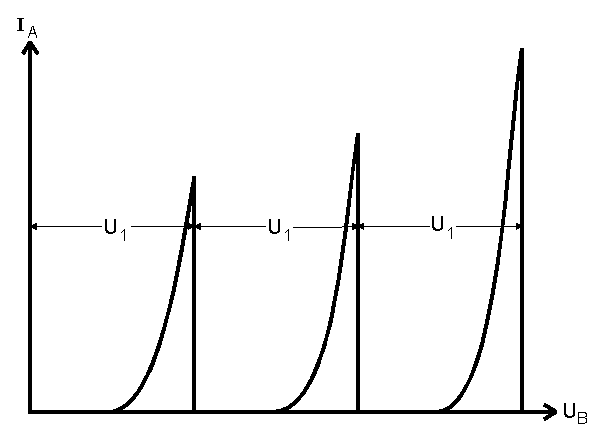
\includegraphics[height = 9cm]{fhkurve.pdf}
    \caption{Abhängigkeit des Auffängerstroms $I_{\symup{A}}$ von der Beschleunigerspannung $U_{\symup{B}}$ \cite{ap601}.}
    \label{fig:fhkurve}
\end{figure}

Der Abstand $U_1$ zwischen aufeinanderfolgenden Maxima stimmt dabei mit dem ersten Anregungspotential überein
\begin{equation}
    U_1 = \frac{1}{e_0}\left(E_1 - E_0\right) \; .
    \label{eqn:U1}
\end{equation}

\subsection{Nebeneffekte mit Einfluss auf die Franck-Hertz-Kurve}
Das Beschleunigungspotential $U_{\symup{B}}$ wird um das Kontaktpotential 
\begin{equation*}
    K = \frac{1}{e_0} \left(\Phi_{\symup{B}}-\Phi_{\symup{G}}\right)
\end{equation*}
reduziert, wenn die Elektroden aus Materialien mit unterschiedlicher Austrittsarbeit bestehen. Um eine hohe Emissionsrate bei niedriger Temperatur zu 
erzielen, wählt man für den Glühdraht ein Material, dessen Austrittarbeit $\Phi_{\symup{G}}$ viel kleiner als die der Beschleunigungselektrode 
$\Phi_{\symup{B}}$ ist.
Außerdem ist die Franck-Hertz-Kurve um den Wert K verschoben.

Desweiteren besitzen die emittierten Elektronen bereits ein Energiespektrum nach der Fermi-Dirac-Verteilung. Dies führt dazu, dass die Elektronen 
mit unterschiedlichen Anfangsgeschwindigkeiten emittiert werden. Daraus entsteht eine Energieverteilung, die bei $U_{\symup{B_eff}}$ beginnt.
Insgesamt wird der Anstieg beim Annähern an das Maximum verringert und die Franck-Hertz-Kurve fällt nicht mehr auf den Wert 0 ab, sondern nu bis 
zu einem Minimum. 
Außerdem führen die elastischen Stöße mit den Hg-Atomen zu Richtungsänderungen der Elektronen, sodass nicht mehr alle Elektronen die Auffängerelektrode 
erreichen. Dies führt insgesamt zu einer Verbreiterung und einer Abflachung der Franck-Hertz-Kurve.

Damit überhaupt Zusammenstöße zwischen Elektronen und Hg-Atomen zustande kommen, muss die mittlere freie Weglänge der Atome
\begin{equation}
    \bar{w} [\symup{cm}] = \frac{0.0029}{p_{\text{sät}} [\symup{mbar}]}
    \label{eqn:weglaenge}
\end{equation}
klein gegenüber dem Abstand a zwischen Glühkathode und Beschleunigungselektrode sein. Dabei ist $p_{\symup{sät}}$ der Sättigungsdampfdruck, der 
aus der Dampfdruckkurve mit
\begin{equation}
    p_{\text{sät}}(T) = 5.5 \cdot 10^7 exp\left(\frac{6876}{T}\right)
    \label{eqn:druck}
\end{equation}
berechnet werden kann. Damit kann eine Temperatur bestimmt werden, bei der der Franck-Hertz-Effekt zu beobachten ist. 

Wenn der Dampfdruckbereich unterschritten wird, durchlaufen die Elektronen ohne Wechselwirkung den Glaskolben. Bei einem zu großen Druck gibt es 
viele elastische Stöße, die zu Richtungsänderungen der Elektronen führen.  

\section{Aufbau}
\label{sec:Aufbau}


\section{Durchführung}
\label{sec:Durchführung}
Der Versuch besteht im wesentlichen aus zwei Teilen. Zwischen jeder neuen Messung muss der XY-Schreiber für die jeweiligen Messungen kalibriert werden.
Hierzu werden die x- und y-Minima so verschoben, dass diese in der unteren linken Bildecke liegen. Auch die Maxima werden so kalibriert, damit eine möglichst große und folglich genau Abbildung dargestellt werden kann.

\subsubsection{Bestimmung der Streuung der Elektronenenergie}
\label{sec:Bestimmung der Streuung der Elektronenenergie}
Der erste Teil des Versuches besteht darin die Streuung der Elektronen zu bestimmen.
Hierzu wird die Beschleunigungsspannung $U_{\text{B}}$ auf einen konstanten Wert gestellt und den X-Eingang des Schreibers die Bremsspannung $U_{\text{A}}$.
Jetzt wird die Bremsspannung erhöht und der XY-Schreiber zeichnet einen Graphen, welcher den vom Picometer gemessenen Strom gegen die Beschleunigungsspannung aufträgt.

\subsubsection{Franck-Hertz-Kurve}
\label{sec:Franck-Hertz-Kurve}
Der zweite Teil besteht darin den Stromverlauf und damit die Anzahl der Ladungen je nach Beschleunigungsspannung graphisch aufzutragen.
An den X-Eingang des Schreibers wird folglich $U_{\text{B}}$ angeschlossen. Die Temperatur $T$ wird auf zwischen $160-200\, \unit{\celsius}$ gestellt und es wird eine konstante Spannung $U_{\text{A}}$ angeschlossen.
Im Anschluss muss $U_{\text{B}}$ gleichmässig erhöht werden, sodass der Schreiber einen Graphen zeichnet. Dieser Vorgang wird bei gleicher Temperatur mit einer anderen Bremsspannung wiederholt.
Nachdem die beiden Graphen gezeichnet wurden, wird die Temperatur erhöht und es werden zwei weitere Graphen gezeichnet.



\section{Auswertung}
\label{sec:Auswertung}

\subsection{Fehlerrechnung}
\label{sec:Fehlerrechnung}
Für die Fehlerrechnung werden folgende Formeln aus der Vorlesung verwendet.
für den Mittelwert gilt
\begin{equation}
    \overline{x}=\frac{1}{N}\sum_{i=1}^N x_i ß\; \;\text{mit der Anzahl N und den Messwerten x} 
    \label{eqn:Mittelwert}
\end{equation}
Der Fehler für den Mittelwert lässt sich gemäß
\begin{equation}
    \increment \overline{x}=\frac{1}{\sqrt{N}}\sqrt{\frac{1}{N-1}\sum_{i=1}^N(x_i-\overline{x})^2}
    \label{eqn:FehlerMittelwert}
\end{equation}
berechnen.
Wenn im weiteren Verlauf der Berechnung mit der fehlerhaften Größe gerechnet wird, kann der Fehler der folgenden Größe
mittels Gaußscher Fehlerfortpflanzung berechnet werden. Die Formel hierfür ist
\begin{equation}
    \increment f= \sqrt{\sum_{i=1}^N\left(\frac{\partial f}{\partial x_i}\right)^2\cdot(\increment x_i)^2}.
    \label{eqn:GaussMittelwert}
\end{equation}


Für die verwendeten Temperaturen ergeben sich mittels \autoref{eqn:druck} der Sättigungsdampfdruck und mittels \autoref{eqn:weglaenge} die mittlere 
freie Weglänge, die beide in \autoref{tab: temp} dargestellt sind.
\begin{table}
    \centering
    \caption{Sättigungsdampfdruck und mittlere freie Weglänge.}
\begin{tabular}{c c c c}
    \toprule
        $T\mathbin{/}\unit{\celsius}$ &$T\mathbin{/}\unit{\kelvin}$ & $p_{\text{sät}}\mathbin{/}\symup{mbar}$ & $\bar{w} \mathbin{/} \unit{\cm}$ \\
    \midrule
    24.2 & 297.35 & 0.0050 & 0.5818\\
    140.2 & 413.35 & 3.2806 & 0.0009\\
    160.9 & 434.05 & 7.2525 & 0.0004\\
    162.1 & 435.25 & 7.5763 & 0.0004\\
    174.8 & 447.95 & 11.8570 & 0.0002 \\
    176.2 & 449.35 & 12.4378 & 0.0002 \\
     \bottomrule
    \end{tabular}
    \label{tab: temp}
\end{table}

Wenn die mittlere freie Weglänge nun mit dem Abstand $a=1\,\unit{\cm}$ zwischen Kathode und Beschleunigerelektrode verglichen wird, stellt man fest, dass die
mittlere freie Weglänge bei den verwendeten Temperaturen weitaus kleiner als dieser ist (Faktor 1000 bis 5000). Bei Zimmertemperatur von $24.2\,\unit{\celsius}$ ist die Differenz
zwischen a und $\bar{w}$ jedoch kleiner, was dazu führt die Stoßwahrscheinlichkeit sehr gering ist.

\subsection{Differentielle Energieverteilung}
Hier werden die ersten beiden Graphen des Anhangs betrachtet, wobei der erste Graph der Messung bei Zimmertemperatur entspricht. Um die Steigung der 
Graphen zu bestimmen, muss zuerst gezählt werden wie viele Skalenteile/Millimeter einem Volt auf der Skala $U_{\symup{A}}$ entsprechen. Dazu werden 
die Abstände zwischen den markierten Skalenpunkten gezählt und im Anschluss gemittelt. Diese Berechnung ist in \autoref{tab:skala1} dargestellt.
\begin{table}
    \centering
    \caption{Einteilung der Skala.}
\begin{tabular}{c c c}
    \toprule
         & Messreihe bei $T=297.35\,\unit{\kelvin}$ & Messreihe bei $T=413.35\,\unit{\kelvin}$ \\
    \midrule
    (0-1)V & 26 Skt & 31 Skt \\
    (1-2)V & 27 Skt & 25 Skt \\
    (2-3)V & 22 Skt & 25 Skt \\
    (3-4)V & 25 Skt & 25 Skt \\
    (4-5)V & 25 Skt & 25 Skt\\
    (5-6)V & 23 Skt &  23 Skt \\
    (6-7)V & 27 Skt & 23 Skt \\
    (7-8)V & 26 Skt & 25 Skt \\
    (8-9)V & 24 Skt & 25 Skt \\
    (9-10)V & 25 Skt & 19 Skt \\
    \midrule
    Mittelwert & 25.0 Skt/V & 24.6 Skt/V \\
     \bottomrule
    \end{tabular}
    \label{tab: temp}
\end{table}

Nun wird für jedes Intervall von 10 Skt die mittlere Steigung abgelesen, indem Steigungsdreiecke eingezeichnet werden. Diese befinden sich bereits auf der 
Abbildung im Anhang. Die Steigungen beider Messreihen befinden sich in \autoref{tab:steigung}.

\begin{table}
    \centering
    \caption{Bestimmung der Steigung der Graphen beider Messreihen.}
\begin{tabular}{c c | c c}
    \toprule
    & Steigung bei $T=297.35\,\unit{\kelvin}$ & & Steigung bei  $T=413.35\,\unit{\kelvin}$ \\
        Position / V & $\frac{\symup{\Delta}y}{\symup{\Delta}x} \mathbin{/} Skt_y/Skt_x$ &Position / V & $\frac{\symup{\Delta}y}{\symup{\Delta}x} \mathbin{/} Skt_y/Skt_x$ \\
    \midrule
    0.16 & 1.9 & 0.2 & 3.0 \\
    0.56 & 1.5 & 0.6 & 1.9 \\
    0.96 & 1.5 & 1.0 & 2.1 \\
    1.36 & 1.4 & 1.4 & 2.0 \\
    1.76 & 1.3 & 1.8 & 1.9 \\
    2.16 & 1.1 & 2.2 & 1.8 \\ 
    2.56 & 1.1 & 2.6 & 1.6 \\
    2.96 & 0.9 & 3.0 & 1.6 \\
    3.36 & 0.9 & 3.4 & 1.4 \\
    3.76 & 0.8 & 3.8 & 1.2 \\
    4.16 & 0.7 & 4.0 & 1.0 \\
    4.56 & 0.7 & &\\
    4.96 & 0.6 & &\\
    5.36 & 0.5 & &\\
    5.76 & 0.4 & &\\
    6.16 & 0.4 & &\\
    6.56 & 0.4 & &\\
    6.96 & 0.3 & &\\
    7.36 & 0.4 & &\\
    7.76 & 0.2 & &\\
     \bottomrule
    \end{tabular}
    \label{tab:steigung}
\end{table}

Die Steigung ist dabei proportional zu der Anzahl der Elektronen, während die Spannung $U_{\symup{A}}$ proportional zu der Energie ist. Für die Messreihe 
bei $T=297.35\,\unit{\kelvin}$ befindet sich die graphische Darstellung der Steigung in Abhängigkeit von der Bremsspannung in \autoref{fig:steigung20}.

\begin{figure}
    \centering
    \includegraphics[width = 12cm]{build/steigung20.pdf}
    \caption{Differentielle Energieverteilung bei $T=297.35\,\unit{\kelvin}$.}
    \label{fig:steigung20}
\end{figure}

Aus dem Graphen in \autoref{fig:steigung20} ergibt sich dabei ein sichtbares Kontaktpotential bei $U_{\symup{A}} = 6.96 \,\unit{\volt}$. Wenn zwischen
$U_{\symup{B}} = 10\,\unit{\volt}$ und diesem Wert eine Differenz gebildet wird, ergibt sich für das Kontaktpotential $K = 3.04\,\unit{\volt}$.

In \autoref{fig:steigung140} wird die Steigung in Abhängigkeit der Spannung $U_{\symup{A}}$ bei $T=413.35\,\unit{\kelvin}$ dargestellt.
\begin{figure}
    \centering
    \includegraphics[width = 12cm]{build/steigung140.pdf}
    \caption{Differentielle Energieverteilung bei $T=413.35\,\unit{\kelvin}$.}
    \label{fig:steigung140}
\end{figure}
Wenn die zweite Messung mit der vorherigen verglichen wird, fällt auf, dass deutlich mehr Elektronen mit Quecksilberatomen stoßen. Um eine qualitative
Aussage, auch bezüglich der Anregungsenergie von Quecksilber, treffen zu können, hätten mehr Messwerte aufgenommen werden müssen, sodass die 
Bremsspannung $U_{\symup{A}}$ auch über die Anregungsenergie von $E = 4.9 \, \symup{eV}$ \cite{anregung} hinausgeht.

\subsection{Franck-Hertz-Kurve} 
Die Franck-Hertz-Kurven bei $U_{\symup{A}} = 1\,\unit{\volt}$ und $U_{\symup{A}} = 2\,\unit{\volt}$ für zwei verschiedene Temperaturen sind ebenfalls 
im Anhang dargestellt.
Es werden erneut für jede Kurve die Skalenteile gezählt un dim Anschluss gemittelt. Für die Kurve bei $U_{\symup{A}} = 1\,\unit{\volt}$ und 
$T = 434.05 \,\unit{\kelvin}$ ergibt sich damit für den Mittelwert $(7.03 \pm 0.08) \symup{Skt/V}$. 
Genauso können die Abstände zwischen den einzelnen Maxima der Franck-Hertz-Kurve abgelesen und gemittelt werden. Diese Daten befinden sich in 
\autoref{tab:fh1max}.
\begin{table}
    \centering
    \caption{Abstände zwischen den Maxima der ersten Franck-Hertz-Kurve.}
\begin{tabular}{c c c}
    \toprule
        Maximum & Abstand in Skt & Abstand $U_1$ in V \\
    \midrule
    1 & 35 \pm 1 & 4.98 \pm 0.06 \\
    2 & 37 \pm 1 & 5.26 \pm 0.06 \\
    3 & 37 \pm 1 & 5.26 \pm 0.06 \\
    4 & 38 \pm 1 & 5.41 \pm 0.06 \\
    \midrule
    Mittelwert & & 5.23 \pm 0.04 \\
     \bottomrule
    \end{tabular}
    \label{tab:fh1max}
\end{table}

Die erste Anregungsenergie des Hg-Atoms ist nun der Mittelwert des Abstands zwischen aufeinanderfolgende Maxima multipliziert mit der Elementarladung
(siehe \autoref{eqn:U1}) 
\begin{equation*}
    (E_1-E_0) = (5.23 \pm 0.04) \,\unit{\eV} \; .
\end{equation*}
Mit \autoref{eqn:nu} und $\lambda = \frac{c}{\nu}$ ergibt sich für die Wellenlänge
\begin{equation*}
    \lambda =  (237.1 \pm 1.8)\,\unit{\nano\meter} \; .
\end{equation*}

Für die weiteren Franck-Hertz-Kurven wird das Verfahren genauso wiederholt.

\subsubsection{Franck-Hertz-Kurve bei $U_{\symup{A}} = 2\,\unit{\volt}$ und $T = 435.25 \,\unit{\kelvin}$}
Der Mittelwert der Skalenteile ergibt sich damit zu $(6.94 \pm 0.08) \symup{Skt/V}$. Die Abstände zwischen den Maxima werden in \autoref{tab:fh2max}
dargestellt.
\begin{table}
    \centering
    \caption{Abstände zwischen den Maxima der zweiten Franck-Hertz-Kurve.}
\begin{tabular}{c c c}
    \toprule
        Maximum & Abstand in Skt & Abstand $U_1$ in V \\
    \midrule
    1 & 37 \pm 1 & 5.04 \pm 0.06 \\
    2 & 38 \pm 1 & 5.33 \pm 0.06 \\
    3 & 42 \pm 1 & 5.48 \pm 0.06 \\
    \midrule
    Mittelwert & & 5.62 \pm 0.06 \\
     \bottomrule
    \end{tabular}
    \label{tab:fh2max}
\end{table}
Die erste Anregungsenergie ergibt sich zu 
\begin{equation*}
    (E_1-E_0) = (5.62 \pm 0.06) \,\unit{\eV} 
\end{equation*}
und die Wellenlänge des emittierten Lichts zu 
\begin{equation*}
    \lambda =  (220.6 \pm 2.4)\,\unit{\nano\meter} \; .
\end{equation*}
\section{Diskussion}
\label{sec:Diskussion}


\newpage
\printbibliography
\nocite{ap601}
\nocite{matplotlib}
\nocite{numpy}
\nocite{scipy}
\nocite{uncertainties}
\nocite{reback2020pandas}

\newpage
%\includepdf[scale=0.9,pages=1,pagecommand=\section*{Anhang}\thispagestyle{empty}]{messdaten.pdf}
%\addcontentsline{toc}{section}{\protect\numberline{}Anhang}
%\includepdf[scale=0.9,pages=2-]{messdaten.pdf}
%\includepdf[pages=-]{messdaten.pdf}

\end{document}
